\chapter{Hardware Developed}
\label{chapter:hardware_developed}
During the development of this thesis, there was both hardware and software developed. In this chapter, the reader will go through the hardware designed to build an appropriate \acrfull{soc} capable of running a full-fledged \acrfull{os}.

The \textit{IOb-SoC} was used as a \acrfull{soc} template. \textit{IOb-SoC} has some features that make it ideal for developing this project \acrshort{soc}. Firstly, it is open-source hardware. Open-source means there are no royalties, and the source code is publicly available. Secondly, adding new peripherals is very easy and intuitive, as was previously seen in section~\ref{subsection:iob_peripherals}. Thirdly, the \textit{IOb-SoC} implements the interface with an internal (SRAM) and an external (DRAM) memory. When using external memory, the \textit{IOb-SoC} instantiates an \textit{iob-cache} system. Finally, the \textit{IOb-SoC} implements a boot hardware unit that controls the first boot stage (also known as stage zero) executed after powering/resetting the system.

The hardware components that needed to be changed from \textit{IOb-SoC} were the \acrfull{cpu} and the \acrfull{uart} peripheral. The \acrshort{cpu} had to be changed because the previous \acrshort{cpu} (\textit{PicoRV32}) could not run a full-featured \acrlong{os}. The author had to swap the \acrshort{uart} since no compatible Linux drivers worked with \textit{iob-UART}. Besides changing a few components from the chip, he had to add new hardware. The new hardware is the \acrshort{clint} and the \acrshort{plic}, both compatible with \textit{RISC-V} specifications. The author created the \acrshort{clint} to support timer and software interrupts on the \acrshort{soc}. He added the \acrshort{plic} to manage interrupts generated by other peripherals. In this project, the \acrshort{uart} is the only additional peripheral that causes an external interrupt. A sketch of the \acrshort{soc} developed can be seen in figure~\ref{fig:bd_linux}.

\begin{figure}[!h]
    \centering
    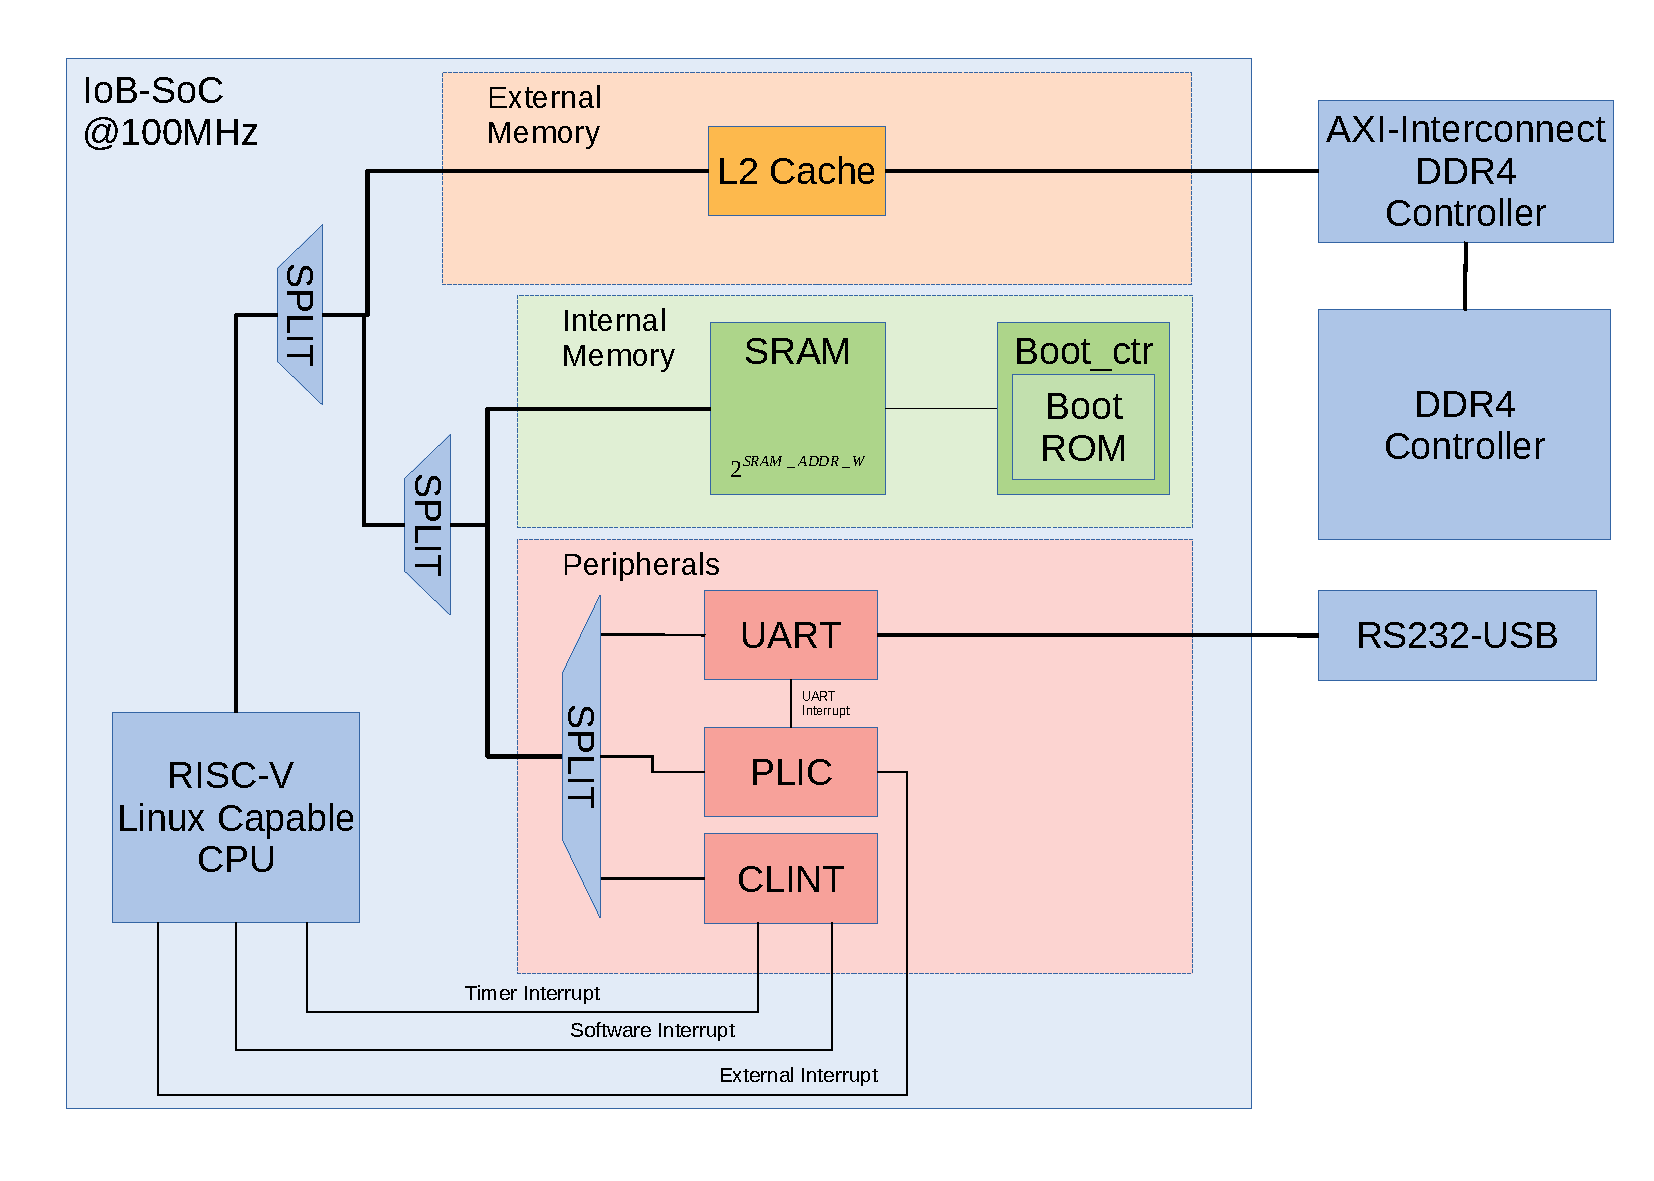
\includegraphics[width=0.7\linewidth]{bd_linux.pdf}
    \caption{Developed \acrshort{soc} sketch.}
    \label{fig:bd_linux}
\end{figure}

Comparing figure \ref{fig:bd_linux} with the original design of \textit{IOb-SoC} (figure \ref{fig:bd_original}) we can see that there were a few additional modifications. In the first place, the reader can see that the candidate removed the L1 Cach. Since every application processor studied had an L1 cache built in, there was no need for the L1 \textit{iob-cache}. Next, a \textit{iob-split} was added to the \textit{IOb-SoC}. Previously, there was a single \textit{iob-split} for the data bus with three branches (the internal memory, the external memory and the peripheral bus). Having three branches meant there were two selection bits; when '00' then, the internal memory bus was active; when '01', it was the peripheral bus; when '10', it was the external memory. Using two bits for selection caused a problem because when addressing the external memory, if its size is bigger than 1GB, the selection bits would be '11'. The \acrfull{demux} output selected by '11' is not connected anywhere, so this caused an internal hardware error. The solution was to include two \textit{iob-split} modules, each with two branches. The first would choose between the external memory and either the internal memory or peripheral bus. The second would choose between the internal memory and the peripheral bus. Another advantage of using this method is that now the selection bit's position does not vary depending on if we are using the DDR or not. Not changing the selection bit makes it easier to use external software that does not use the \textit{iob-soc} Makefiles. Before, the peripheral addressing on external software had to be changed every time the developer wanted to test with or without the external memory.

\section{Central Processing Unit}
\label{section:cpu}
The \acrshort{cpu} chosen to use in this project was \textit{VexRiscv}~\cite{vexriscv}. The performance of the CPU is not a significant issue for this project. However, how the developers designed the core highly influenced the CPU decision. The flexibility of the CPU design, meaning how easily the CPU can be adapted to take advantage of the other components in \textit{IOb-SoC}, is an essential factor. Since the hardware and software developed in this project are open-source, the CPU implemented had to be open-source hardware. Moreover, knowing that the \textit{IOb-SoC} signals are 32-bit wide, ideally, the selected CPU should support RV32IMAC to facilitate its integration with IOb-SoC. From the \acrshort{cpu}s studied in chapter \ref{chapter:existing_embedded_technologies} \textit{VexRiscv} looked like the more indicated.

Generating the \acrshort{rtl} \textit{verilog} file from the \textit{SpinalHDL} hardware description is very simple. After cloning the \textit{VexRiscv}, GitHub repository, the developer only has to run one command. As can be seen below in listing \ref{lst:rtl_vexriscv}. On the \textit{VexRiscv} repository there exist a couple of demo \acrshort{cpu} configurations. The developers can use configurations directly or configure them to generate a custom \textit{VexRiscv} core. There even already exists a demo configuration to generate a Linux-compatible core. Although the author implemented a custom core, he used the Linux demo configuration as a starting point. Unfortunately, the Linux Demo design is outdated, and the instructions, commented on the hardware configuration file, to run a Linux simulation and test the core does not work.

\begin{lstlisting}[language=make, caption={Generate \textit{verilog} from \textit{SpinalHDL}}, label=lst:rtl_vexriscv]
git clone https://github.com/SpinalHDL/VexRiscv.git && \
  cd VexRiscv && sbt "runMain vexriscv.demo.LinuxGen"
\end{lstlisting}

Developers can configure the \textit{VexRiscv} by adding and removing plugins. Plugins are hardware components described in \textit{SpinalHDL} that can be reused in different designs by simply adding \enquote{\textcolor{green}{new} \textcolor{red}{Plugin\_Name}(...),} to the plugins list in the top \acrshort{cpu} description file. The existing plugins are described in the \textit{VexRiscv} repository on the \enquote{src/main/scala/vexriscv/plugin} directory. The available plugins show developers two different plugins for the instruction bus and another two for the data bus. They are \enquote{IBusSimplePlugin}, \enquote{IBusCachedPlugin}, \enquote{DBusSimplePlugin} and \enquote{DBusCachedPlugin}. The difference is that the \enquote{cached} plugins have the L1 Cache integrated, while the simple plugins do not. An additional difference between the data cached and simple plugin is that, although the \enquote{DBusCachedPlugin} fully supports both, the \enquote{DBusSimplePlugin} supports only \acrfull{lr}/\acrfull{sc} but not \acrfull{amo} instructions. The \enquote{DBusSimplePlugin} could also be adapted to enable the full \enquote{A} extension. However, knowing how to write in \textit{SpinalHDL} would be necessary. Learning how to code in \textit{SpinalHDL} would be very time-consuming and not in this project's scope.

The first step on implementing the \textit{VexRiscv} core on the \textit{IOb-SoC} was making sure that it worked on \enquote{bare metal} applications. The developed \acrshort{soc} had to work with the application accessing the silicon chip directly without any intermediary like an \acrfull{os}. The author first developed the \acrshort{soc} for \enquote{bare metal} applications using the instruction and data \enquote{simple} plugins. The next step was to run the Linux kernel. To do so, the instruction and data \enquote{simple} plugins had to be changed to the \enquote{cached} plugins. The missing support for \acrfull{amo} instructions was noticeable because the software would stop executing and enable an unknown instruction signal. The signal waves created during the simulation made it possible to identify which instruction was causing the problem.

The final \textit{VexRiscv} core configuration file contained the needed plugins to run a minimal \acrfull{os} based on Linux. The plugins present were:
% The file can be found in the project git hub repository under (\url{https://github.com/IObundle/iob-vexriscv/blob/cached_vexriscv/software/vexriscv_core/Linux.scala}).
\begin{itemize}
  \item The \enquote{IBusCachedPlugin} was added. With it, developers could define the address of the first instruction the CPU had to fetch by setting the reset value of the \acrfull{pc}. In this plugin, developers could also specify if the CPU had a branch predictor and if it supported compressed instructions. 
  \item The \enquote{DBusCachedPlugin} was added for the reason that it fully supported the atomic instructions.
  \item The \enquote{DecoderSimplePlugin} is used to decode the instructions.
  \item The \enquote{RegFilePlugin} implements the register file. These are the registers inside the CPU.
  \item The \enquote{IntAluPlugin} is used to calculate arithmetic and logic operations.
  \item The \enquote{SrcPlugin} is an auxiliary plugin for the plugins that contain \acrfull{alu}, Branch related hardware and Load/Store hardware logic.
  \item The \enquote{FullBarrelShifterPlugin} implements the shift instructions present in the \textit{RISC-V} base \acrfull{isa}.
  \item The \enquote{HazardSimplePlugin} determines where the core needs to stall.
  \item The \enquote{MulPlugin} allows the core to execute multiplication instructions.
  \item The \enquote{MulDivIterativePlugin} could be used to add multiplication and division support to the core (\textit{RISC-V} M \acrshort{isa} extension). In this project, the author used it to add only division since another plugin added multiplication support.
  \item The \enquote{CsrPlugin} is configured to support Linux fully. This plugins adds the needed \acrfull{csr} to run a full feature \acrshort{os}.
  \item The \enquote{BranchPlugin} allows the core to execute and make decisions on the jump instructions. Jump instructions are part of the base \acrfull{isa}
  \item The \enquote{MmuPlugin} added support for the \acrfull{mmu}. Which is required to run a full feature \acrshort{os}.
\end{itemize}

For this project, the author decided not to use any branch predictor since the performance of the \acrshort{soc} was not a concern. Furthermore, there seemed to be a compatibility problem between the most recent \textit{RISC-V} toolchain and the branch predictors available in the \textit{VexRiscv}. Additional, he decided that \acrshort{cpu} should support compressed instructions because compressed instructions allowed to reduce the firmware size considerably. 

The author could have used some additional plugins. The \enquote{DebugPlugin} could be used to debug the CPU core if a JTAG interface existed. However, the \textit{IOb-SoC} does not support it. The \enquote{FpuPlugin} can add support for both the floats and doubles instructions. In the core used, this plugin was deactivated since to run a minimal \acrshort{os}, there is little to no advantage of using this extension, causing the FPU only to be adding unnecessary hardware logic.

After generating the Verilog file that describes a \textit{VexRiscv} core, the author had to create a wrapper hardware module that adapted the \textit{VexRiscv} core interface to the \textit{IOb-SoC} internal bus.

\section{VexRiscv Wrapper}
The Verilog wrapper, witch is called \textit{iob\_VexRiscv}, is instantiated by the \textit{IOb-SoC} top \acrshort{soc} hardware module as the \acrshort{cpu} component and instantiates the \textit{VexRiscv} core Verilog module. The author created an interface between the \textit{IOb-SoC} hardware and the \textit{VexRiscv} core by establishing a connection between the inputs and outputs from both sides.

The \textit{iob\_vexriscv} has multiple input signals. The clock signal is the system clock derivative from the development board where the users implement the \acrshort{soc}. The reset signal is set to high ('1') when the system reboots or the stage 0 bootloader finishes. The boot signal has the value '1' while the stage 0 bootloader is executing. After it finishes, the boot signal value drops to '0' while the hardware sets the reset signal to high. The instruction bus response signal is connected to \enquote{cpu\_i\_resp}. The data bus response signal is connected to \enquote{cpu\_d\_resp}. The timer interrupt and software interrupt signals are '1' or '0' depending on the outputs from the \acrshort{clint} unit. Lastly, the \acrshort{plic} unit controls the external interrupt input signal. The output signals are the instruction bus request signal and the data bus request signal, which connect to the \enquote{cpu\_i\_req} and \enquote{cpu\_d\_req} respectably. The \enquote{cpu\_i\_resp}, \enquote{cpu\_d\_resp}, \enquote{cpu\_i\_req} and \enquote{cpu\_d\_req} signals correspond to the request and response buses reviewed in section \ref{subsection:iob_bus}.

The input and output signals of the \textit{VexRiscv} core can be seen in table \ref{tab:vexriscv_core_and_iob_soc}. The reader can also see the signal's width and their equivalent signal in the \textit{IOb-SoC} top hardware.

\begin{table}[!ht]
  \centering
  \resizebox{\textwidth}{!}{%
  \begin{tabular}{|l|l|l|l|l|}
    \hline
    \textbf{Port}                & \textbf{Width} & \textbf{Direction} & \textbf{Description}                                                                                          & \textbf{IOb-SoC Port}           \\ \hline
    dBus\_cmd\_valid             & 1              & output             & \begin{tabular}[c]{@{}l@{}}Indicates that the CPU is ready\\  to make a data request.\end{tabular}            & cpu\_d\_req{[}`valid(0){]}      \\ \hline
    dBus\_cmd\_ready             & 1              & input              & \begin{tabular}[c]{@{}l@{}}Indicates that the SoC is ready\\  to receive a data request.\end{tabular}         & N/A                             \\ \hline
    dBus\_cmd\_payload\_wr       & 1              & output             & \begin{tabular}[c]{@{}l@{}}Indicates that the CPU wants\\  to write data to memory.\end{tabular}              & N/A                             \\ \hline
    dBus\_cmd\_payload\_uncached & 1              & output             & Indicates if data is on L1 cache                                                                              & Not used                        \\ \hline
    dBus\_cmd\_payload\_address  & 32             & output             & Used to address memory.                                                                                       & cpu\_d\_req{[}`address(0,32){]} \\ \hline
    dBus\_cmd\_payload\_data     & 32             & output             & Used to send data to memory.                                                                                  & cpu\_d\_req{[}`wdata(0){]}      \\ \hline
    dBus\_cmd\_payload\_mask     & 4              & output             & \begin{tabular}[c]{@{}l@{}}Indicates which bytes in a\\  word are accessed.\end{tabular}                      & N/A                             \\ \hline
    dBus\_cmd\_payload\_size     & 2              & output             & $log_2$(number of bytes in the burst)                                                                         & Not used                        \\ \hline
    dBus\_cmd\_payload\_last     & 1              & output             & \begin{tabular}[c]{@{}l@{}}Indicates when the last\\  byte is transferred.\end{tabular}                       & Not used                        \\ \hline
    dBus\_rsp\_valid             & 1              & input              & \begin{tabular}[c]{@{}l@{}}Indicates that the SoC is ready\\  to send a response.\end{tabular}                & cpu\_d\_resp{[}`valid(0){]}     \\ \hline
    dBus\_rsp\_payload\_last     & 1              & input              & \begin{tabular}[c]{@{}l@{}}Indicates when the last\\  byte is transferred.\end{tabular}                       & Not used                        \\ \hline
    dBus\_rsp\_payload\_data     & 32             & input              & Receive data from memory.                                                                                     & cpu\_d\_resp{[}`rdata(0){]}     \\ \hline
    dBus\_rsp\_payload\_error    & 1              & input              & Indicates existence of an error.                                                                              & Not used                        \\ \hline
    timerInterrupt               & 1              & input              & Indicate a Timer Interrupt.                                                                                   & timerInterrupt                  \\ \hline
    externalInterrupt            & 1              & input              & Indicate an External Interrupt.                                                                               & externalInterrupt               \\ \hline
    softwareInterrupt            & 1              & input              & Indicate a Software Interrupt.                                                                                & softwareInterrupt               \\ \hline
    externalInterruptS           & 1              & input              & \begin{tabular}[c]{@{}l@{}}Indicate an External Interrupt\\  at the Supervisor level.\end{tabular}            & Not used                        \\ \hline
    iBus\_cmd\_valid             & 1              & output             & \begin{tabular}[c]{@{}l@{}}Indicates that the CPU is ready\\  to make an instruction request.\end{tabular}    & cpu\_i\_req{[}`valid(0){]}      \\ \hline
    iBus\_cmd\_ready             & 1              & input              & \begin{tabular}[c]{@{}l@{}}Indicates that the SoC is ready\\  to receive an instruction request.\end{tabular} & N/A                             \\ \hline
    iBus\_cmd\_payload\_address  & 32             & output             & Used to address memory.                                                                                       & cpu\_i\_req{[}`address(0,32){]} \\ \hline
    iBus\_cmd\_payload\_size     & 2              & output             & $log_2$(number of bytes in the burst)                                                                         & Not used                        \\ \hline
    iBus\_rsp\_valid             & 1              & input              & \begin{tabular}[c]{@{}l@{}}Indicates that the SoC is ready\\  to send a response.\end{tabular}                & cpu\_i\_resp{[}`valid(0){]}     \\ \hline
    iBus\_rsp\_payload\_data     & 32             & input              & Receive an instruction from memory.                                                                           & cpu\_i\_resp{[}`rdata(0){]}     \\ \hline
    iBus\_rsp\_payload\_error    & 1              & input              & Indicates existence of an error.                                                                              & Not used                        \\ \hline
    clk                          & 1              & input              & System clock signal.                                                                                          & clk                             \\ \hline
    reset                        & 1              & input              & CPU reset signal.                                                                                             & cpu\_reset                      \\ \hline
    \end{tabular}%
  }
  \caption{\textit{VexRiscv} core inputs and outputs.}
  \label{tab:vexriscv_core_and_iob_soc}
\end{table}

After understanding the inputs and outputs of each module, it is easy to see which wires should be connected. However, after connecting all the wires, there were three problems. The first was the \enquote{strb} signal needed by \textit{IOb-SoC} when writing data to memory which did not exist in the \textit{VexRiscv} signals. The author could obtain the \enquote{strb} signal in two different ways. One way would be through the \enquote{dbus\_req\_size} signal, the two less significant bits of the \enquote{dbus\_req\_address} and the \enquote{dbus\_req\_wr} signal. The other way was through the \enquote{dBus\_cmd\_payload\_mask} signal and the \enquote{dBus\_cmd\_payload\_wr} signal. The \enquote{DBusSimplePlugin}, contrary to the \enquote{DBusCachedPlugin}, had no \enquote{dBus\_cmd\_payload\_mask} signal that is why the first method was created. Accordingly, for the first method, the \enquote{mask} signal had to be generated by the hardware logic expressed in equation \ref{eq:mask_generated}. % Should I make a figure with a MUX and a shifter?

\begin{equation}
  \begin{cases}
    dbus\_req\_mask\_aux = dbus\_req\_size[1] ? {4'hF} : (dbus\_req\_size[0] ? {4'h3} : {4'h1}) \\
    dbus\_req\_mask = dbus\_req\_mask\_aux << dbus\_req\_address[1:0]
  \end{cases}
  \label{eq:mask_generated}
\end{equation}

Moreover, the \enquote{mask} signal indicated the active bytes when both read or write operations were occurring. On the other hand, the \enquote{strb} signal should only be active when a write operation is happening. Both methods logic expressions can be seen in equation \ref{eq:strb_vexriscv}. This implements a \acrshort{mux} where \enquote{dbus\_req\_wr} is the selection bit.

\begin{equation}
  \begin{split}
  strb& = dbus\_req\_wr ? dbus\_req\_mask : 4'h0 \\
      & = dbus\_req\_wr ? dBus\_cmd\_payload\_mask : 4'h0
  \end{split}
  \label{eq:strb_vexriscv}
\end{equation}

The second is that the \textit{IOb-SoC} internal bus did not contain all the signals needed by the \textit{VexRiscv} core. To successfully make the interface handshake with the \textit{VexRiscv} core, the candidate had to generate an instruction and data request \enquote{ready} signal. The \enquote{ready} signal indicated that the \acrshort{soc} was ready to receive and accept a request from the CPU. To solve this problem a register that saved the value of the \enquote{cmd\_valid}, called \enquote{valid\_reg}, was created. This register would be updated when either the \enquote{cmd\_valid} or the \enquote{rsp\_valid} signal were active. The \enquote{ready} signal should be high ('1') before accepting a request, and after, it should be low ('0') while the response is not available. The initial approach to the values that the \enquote{cmd\_ready} signal should assume can be seen in the truth table \ref{tab:first_truth_table}. The candidate obtained this truth table by analysing the simulation signals wave. The \enquote{N/A} values in the table mean that those situations never occurred.

\begin{table}[!h]
  \centering
  \begin{tabular}{ccc|c}
  valid\_reg & cmd\_valid & rsp\_valid & cmd\_ready \\ \hline
  0          & 0          & 0          & 0          \\
  0          & 0          & 1          & N/A        \\
  0          & 1          & 0          & 1          \\
  0          & 1          & 1          & N/A        \\
  1          & 0          & 0          & 0          \\
  1          & 0          & 1          & 1          \\
  1          & 1          & 0          & 0          \\
  1          & 1          & 1          & 1         
  \end{tabular}
  \caption{First try at identifying the rules the cmd\_ready should follow.}
  \label{tab:first_truth_table}
\end{table}

Engineers can transform the truth table into a logic gates expression, and the reader can see the expression in equation \ref{eq:first_logic_eq}.

\begin{equation}
  (valid\_reg \cdot rsp\_valid) + (valid \cdot \overline{valid\_reg} \cdot \overline{rsp\_valid})
  \label{eq:first_logic_eq}
\end{equation}

However, this approach had an issue. The logic expression depended on the \enquote{cmd\_valid} signal which was generated inside the \textit{VexRiscv} core. Depending on the \enquote{cmd\_valid} signal could generate a bigger complication since the combinatorial circuit that generates the \enquote{cmd\_valid} is unknown and might generate an infinite hardware loop. From better analyzing the signal behavior it was noticed that when \enquote{valid\_reg}, \enquote{cmd\_valid} and \enquote{rsp\_valid} are low ('0') the value of \enquote{cmd\_ready} is irrelevant. It could be concluded since when the \enquote{valid\_reg}, \enquote{cmd\_valid} and \enquote{rsp\_valid} are low happens the \enquote{cmd\_ready} signal was not being used by the \textit{IOb-SoC}. The truth table can them be simplified to table \ref{tab:simple_truth_table}.

\begin{table}[!ht]
  \centering
  \begin{tabular}{cc|c}
  valid\_reg & rsp\_valid & req\_ready \\ \hline
  0          & 0          & 1          \\
  0          & 1          & N/A        \\
  1          & 0          & 0          \\
  1          & 1          & 1         
  \end{tabular}
  \caption{Simplified truth table.}
  \label{tab:simple_truth_table}
\end{table}

Engineers can see the truth table \ref{tab:simple_truth_table} as a simple XOR logic gate. The equation \ref{eq:simple_logic_eq} represents the hardware logic expression implement.

\begin{equation}
  (valid_reg \cdot rsp\_valid) + (\overline{valid_reg} \cdot \overline{rsp\_valid}) = valid_reg \odot rsp\_valid
  \label{eq:simple_logic_eq}
\end{equation}

The last problem was that after accepting an instruction or data request the values of the \enquote{address}, \enquote{data} and \enquote{mask} signals could change inside the \textit{VexRiscv} core. This changes would pass through \textit{iob\_VexRiscv} and reflect in the rest of \textit{IOb-SoC} hardware. Which caused the \textit{iob-cache} and peripherals to not function currently. The author solved this problem by creating registers that saved the value of the \enquote{address}, \enquote{data} and \enquote{strb} signals when the request was accepted. The register values would then only change when the response was already received.

Finally, the \acrshort{cpu} should be able to run firmware from both the internal and external memory. When the stage 0 bootloader is running, the hardware has to force the \acrfull{msb} of the instruction fetch address to '0'. Having the \acrshort{msb} set to ‘0’ forces the \acrshort{cpu} to fetch instructions from the boot hardware unit. When the user defines the firmware to run from the external memory (\enquote{RUN\_EXTMEM=1}), the first instruction fetched should be at address $0x80000000$. When \enquote{RUN\_EXTMEM=1}, the wrapper defined the \acrfull{msb} as the negated value of the boot signal. When \enquote{RUN\_EXTMEM=0}, the Verilog forced the \acrshort{msb} to be '0' since there is no need to access the external memory. On the data request bus, it should also be taken into account that the \acrshort{msb} had to be '0' when the \acrshort{cpu} wanted to access the peripherals.

\section{\textit{UART 16550}}
\label{section:uart}
The approach taken in this project was to adapt an existing open-source \acrfull{uart} core that the Linux kernel supports. The other option was to create a Linux driver compatible with \textit{iob-UART} and compile it with the kernel. The chosen approach seemed an adequate and more straightforward solution.

Since the developed chip is supposed to be open-source, the \acrshort{uart} core should also be open-source hardware. The core used was a \textit{\acrshort{uart}16550}~\cite{gorban2002uart} that has been made available by \textit{freecores} on \textit{github}. The developers of the \textit{\acrshort{uart}16550} wrote it in Verilog. Although it was an older version of Verilog, it is still synthesisable by modern tools and easy to understand. The \textit{UART16550} core used implements a wishbone interface to interact with the \acrfull{soc}. Similarly to what the author did with the CPU, he had to create a wrapper to adapt the core to the \textit{IOb-SoC}.

The \textit{UART16550} developers defined the wishbone interface in the top hardware module of their \acrshort{uart} core. In table \ref{tab:uart16550_wishbone}, which can be obtained from the open-source \textit{UART16550} core documentation, it can be seen the wishbone interface signals. The wishbone specification determines that there needs to be a master and a slave. In this case when the \acrshort{cpu} sends a request signal for the \textit{UART16550} peripheral the master is the \acrshort{cpu} and the slave is the \textit{UART16550}.

\begin{table}[!ht]
  \centering
  \begin{tabular}{|l|l|l|l|}
  \hline
  \textbf{Port} & \textbf{Width} & \textbf{Direction} & \textbf{Description}          \\ \hline
  CLK           & 1              & Input              & Block's clock input           \\ \hline
  WB\_RST\_I    & 1              & Input              & Asynchronous Reset            \\ \hline
  WB\_ADDR\_I   & 5 or 3         & Input              & Used for register selection   \\ \hline
  WB\_SEL\_I    & 4              & Input              & Select signal                 \\ \hline
  WB\_DAT\_I    & 32 or 8        & Input              & Data input                    \\ \hline
  WB\_DAT\_O    & 32 or 8        & Output             & Data output                   \\ \hline
  WB\_WE\_I     & 1              & Input              & Write or read cycle selection \\ \hline
  WB\_STB\_I    & 1              & Input              & Specifies transfer cycle      \\ \hline
  WB\_CYC\_I    & 1              & Input              & A bus cycle is in progress    \\ \hline
  WB\_ACK\_O    & 1              & Output             & Acknowledge of a transfer     \\ \hline
  \end{tabular}
  \caption{WISHBONE interface signals.}
  \label{tab:uart16550_wishbone}
\end{table}

The interface between the \textit{IOb-SoC} and the \textit{UART16550} top hardware is established by the Verilog module that acts as a \textit{UART16550} wrapper. The wrapper module is called \enquote{iob\_uart16550}. The \enquote{iob\_uart16550} hardware component has to generate the missing signals that the wishbone interface requires but do not exist in \textit{IOb-SoC}. In table \ref{tab:wishbone_iob_soc} the connection between the \textit{IOb-SoC} and the \textit{UART16550} wishbone interface can be analyzed. The missing signal are the \enquote{WB\_SEL\_I}, the \enquote{WB\_WE\_I} and the \enquote{WB\_STB\_I}. The select signal is similar to the \enquote{strb} signal but should exist during write and read operations. The hardware can obtain this signal through the address signal's two \acrfull{lsb}. Furthermore, since registers are addressed byte by byte, only one bit at a time will be set to high on the select signal. When the \acrshort{cpu} wants to write to the \textit{UART16550} registers, the hardware has to set the write signal high. This can be perceived through the \textit{IOb-SoC} \enquote{strb} signal. If any of the \enquote{strb} bits are enabled the \enquote{WB\_WE\_I} signal should be high ('1'). The transfer cycle should happen (i.e. the wrapper should set the \enquote{WB\_STB\_I} signal should '1') when the \textit{UART16550} has accepted a request but still has not issued the response. Furthermore, the \textit{UART16550} has an interrupt output pin that is connected to the \acrshort{soc} \enquote{uartInterrupt}. The \acrshort{soc} \enquote{uartInterrupt} is then passed to the \acrshort{plic} unit.

\begin{table}[!ht]
  \centering
  \resizebox{\textwidth}{!}{%
  \begin{tabular}{|l|l|l|}
  \hline
  \textbf{UART16550 Wishbone} & \textbf{IOb-UART16550}                  & \textbf{IOb-SoC}                         \\ \hline
  CLK                         & clk                                     & clk                                      \\ \hline
  WB\_RST\_I                  & rst                                     & reset                                    \\ \hline
  WB\_ADDR\_I                 & address{[}`UART\_ADDR\_WIDTH-1:0{]}     & slaves\_req{[}`address(`UART16550,32){]} \\ \hline
  WB\_SEL\_I                  & 1\textless{}\textless{}address{[}1:0{]} & N/A                                      \\ \hline
  WB\_DAT\_I                  & wdata                                   & slaves\_req{[}`wdata(`UART16550){]}      \\ \hline
  WB\_DAT\_O                  & rdata                                   & slaves\_resp{[}`rdata(`UART16550){]}     \\ \hline
  WB\_WE\_I                   & | wstrb                                 & N/A                                      \\ \hline
  WB\_STB\_I                  & valid\&($\sim$ready)                    & N/A                                      \\ \hline
  WB\_CYC\_I                  & valid                                   & slaves\_req{[}`valid(`UART16550){]}      \\ \hline
  WB\_ACK\_O                  & ready                                   & slaves\_resp{[}`ready(`UART16550){]}     \\ \hline
  \end{tabular}%
  }
  \caption{\textit{UART16550} interface with \textit{IOb-SoC}.}
  \label{tab:wishbone_iob_soc}
\end{table}

Finally, the \enquote{iob\_uart16550} also has to pass the interface between the \textit{UART16550} core and the RS232 connector. That is why it implements the: txd output to transmit data through serial; the rxd input to receive data through serial; the cts input, which indicates that the destination is ready to receive a transmission sent by the UART; the rts output, which indicates that the UART is ready to receive a transmission from the sender. The \acrshort{fpga} connects those pins to the development board RS232 connector.

\section{CLINT Unit}
\label{section:clint}
The \acrshort{clint} was the only hardware component developed from scratch. Even though there already exist open-source \acrfull{clint} hardware modules. For example, the \acrshort{clint} used with the \textit{CVA6} core and developed by the \textit{PULP platform}. The problem with this \acrshort{clint} module is that it is written in system-Verilog and uses packages and definitions from the \textit{CVA6} core. The \acrshort{clint} core is a simple hardware component that only needs a few registers and signals to work. The author would have to create an interface with \textit{IOb-SoC} independently of the \acrshort{clint} core used. The best solution was to entirely create the \acrshort{clint} hardware unit.

Table \ref{tab:clint_registers} shows the memory mapped register and their respective address implemented on the developed \acrshort{clint} hardware. The \acrshort{clint} registers are compatible with both the \textit{SiFive} and the \textit{RISC-V} specification. Since the \acrshort{soc} developed only has one Hart (i.e. \acrshort{cpu} core), the Verilog code only creates one register of each type, three registers in total. Nevertheless, the register's address must be separate because developers could use the \acrshort{clint} created by the author in more complex systems. Furthermore, the logic behaviour of the \acrshort{clint} hardware is identical to the behaviour described in the \textit{RISC-V} specification reviewed in section \ref{subsection:clint_riscv}.

\begin{table}[!ht]
  \centering
  \begin{tabular}{|l|l|l|l|l|}
  \hline
  \textbf{Name} & \textbf{Address} & \textbf{Width (bit)} & \textbf{Access} & \textbf{Description}                    \\ \hline
  MSIP          & 0x0              & 32                   & RW              & Software interrupt                      \\ \hline
  MTIMECMP      & 0x4000           & 64                   & RW              & Register to compare with timer register \\ \hline
  MTIME         & 0x1bff8          & 64                   & RW              & Timer register                          \\ \hline
  \end{tabular}
  \caption{CLINT Registers.}
  \label{tab:clint_registers}
\end{table}

The inputs and outputs of the \acrshort{clint} unit can be seen in table \ref{tab:clint_signals}. \enquote{N\_CORES} is the number of \acrshort{cpu} core that are used in the \acrshort{soc}. In the \acrfull{soc} developed, there is only one core. Nevertheless, the author built the \acrshort{clint} considering a possibility of a multi-core system. Each core has its timer and software interrupt. As such, the \enquote{mtip} and \enquote{msip} signals width is the number of core, \enquote{N\_CORES}. When the \acrshort{clint} hardware receives a request from the \acrshort{cpu}, the response is ready one clock cycle after. The response data will be the data stored in the register designated by the request address signal. If the request strobe signal is different from 0, then the \acrshort{clint} writes to the register the request addresses. The value stored in that register will be the same as the request data signal.

\begin{table}[!ht]
  \centering
  \resizebox{\textwidth}{!}{%
  \begin{tabular}{|l|l|l|l|l|}
  \hline
  \textbf{Port} & \textbf{Width} & \textbf{Direction} & \textbf{Description}                                                                                & \textbf{IOb-SoC Port}                \\ \hline
  clk           & 1              & input              & System clock                                                                                        & clk                                  \\ \hline
  rst           & 1              & input              & System reset                                                                                        & reset                                \\ \hline
  rt\_clk       & 1              & input              & Real-time clock                                                                                     & rtc                                  \\ \hline
  valid         & 1              & input              & \begin{tabular}[c]{@{}l@{}}Indicates that the CPU is ready\\   to make a data request.\end{tabular} & slaves\_req{[}`valid(`CLINT){]}      \\ \hline
  address       & 32             & input              & Register address.                                                                                   & slaves\_req{[}`address(`CLINT,16){]} \\ \hline
  wdata         & 32             & input              & Data to write to register.                                                                          & slaves\_req{[}`wdata(`CLINT){]}      \\ \hline
  wstrb         & 4              & input              & Used to generate a "write" signal.                                                                  & slaves\_req{[}`wstrb(`CLINT){]}      \\ \hline
  rdata         & 32             & output             & Data read from register.                                                                            & slaves\_resp{[}`rdata(`CLINT){]}     \\ \hline
  ready         & 1              & output             & \begin{tabular}[c]{@{}l@{}}Indicates that the CLINT is ready\\   to send a response.\end{tabular}   & slaves\_resp{[}`ready(`CLINT){]}     \\ \hline
  mtip          & N\_CORES       & output             & Raise a timer interrupt in a core.                                                                  & timerInterrupt                       \\ \hline
  msip          & N\_CORES       & output             & Raise a software interrupt in a core.                                                               & softwareInterrupt                    \\ \hline
  \end{tabular}%
  }
  \caption{CLINT interface with \textit{IOb-SoC}.}
  \label{tab:clint_signals}
\end{table}

The \enquote{rt\_clk} signal, although it is connected to \enquote{rtc} wire, is not available in \textit{IOb-SoC} since the development board does not have any \acrfull{rtc} crystal connected. The \acrshort{rtc} frequency is commonly 32.768 kHz, because it is a power of 2 ($2^15$) value. To get a precise 1-second period (1 Hz frequency) would only be needed a 15 stage binary counter. With a \acrshort{rtc} the \acrshort{clint} unit had to detect the rising edge of the \enquote{rt\_clk} signal. The hardware detected the rising edge by taking samples of the \enquote{rt\_clk} signal at the system clock frequency. Taking those samples is possible because the \acrshort{rtc} is slower than the system clock. Suppose in the future, the \acrshort{clint} unit developed is implemented in a system with a \acrshort{rtc}. In that case, developers can easily adapt the hardware design to support the \acrshort{rtc} since the author developed the logic.

The development boards used in this thesis do not have an \acrshort{rtc}, so the author had to find an alternative. The method implemented was more straightforward than the logic if a \acrshort{rtc} existed. The system clock operates at 100 MHz, so the author added a counter to the design that increases the timer register when the counter reaches a defined threshold. The \acrshort{clint} timer frequency the author defined is 100KHz and the Verilog code calculates the counter threshold with $\frac{SystemFrequency}{100000}-1$. Therefore, if the system frequency is 100MHz, the hardware simulates a \acrshort{rtc} working at 100 kHz by incrementing the timer when the counter reaches 999.

\section{PLIC Unit}
\label{section:plic}
The \acrshort{plic} is not essential to run a full feature \acrfull{os} on a \acrfull{soc}. Since the \acrshort{soc} uses the \acrshort{plic} to drive interrupts generated by other peripherals to the \acrshort{cpu}, in this project, the only peripheral connected to the \acrshort{plic} is the \textit{UART16550}. For the growth of the \acrshort{soc}, the \acrshort{plic} unit is a handy requirement. Developers in the future can add some peripherals that also use the \acrshort{plic} hardware. For example, the \textit{ethernet} controller can be used to wake a core from low power mode.

Since the \acrshort{plic} hardware unit is more complex then the \acrshort{clint}, it was decided that an open-source \acrshort{plic} core would be adapted to the \textit{IOb-SoC}. There were three available cores. The \acrshort{plic} developed by \textit{lowRISC}~\cite{lowrisc_plic} is written in their own variation of \textit{System Verilog}, consequently it is difficult to adapt and test in simulation. The \acrshort{plic} used with the \textit{CVA6} core, developed by the \textit{PULP platform}~\cite{pulp_plic}, started as a fork of an older version of the \textit{lowRISC}. This \acrshort{plic} unit is written in traditional \textit{System Verilog}. I tried to adapt the \acrshort{plic} unit from \textit{PULP platform} but there were many incompatibilities with the \textit{IOb-SoC}. Finally, the \acrshort{plic} developed by \textit{RoaLogic}~\cite{roalogic_plic} was the hardware unit used as a starting point. The \textit{RoaLogic} \acrshort{plic} is also written in \textit{System Verilog} and implements an \textit{apb4} or \textit{ahb3lite} interface with the \acrshort{soc}. The biggest advantage of the \textit{RoaLogic} hardware is that the \acrshort{plic} relevant components for the \textit{IOb-SoC}, the \acrshort{plic} registers and core, are well separated from the modules that create the interface with the \acrshort{soc} and instantiate them. To integrate the a \acrshort{plic} unit on the \textit{IOb-SoC} I had to develop a \acrshort{plic} wrapper.

The \acrshort{plic} wrapper had to create the interface with the \textit{IOb-SoC} internal buses. Furthermore, it needed to instantiate the \acrshort{plic} registers and core hardware modules.

The \acrshort{plic} hardware module was named \enquote{iob\_plic}. When instantiating the \enquote{iob\_plic}, there are various parameters the developer can customise that influence the hardware. The number of interrupt sources defines how many peripheral interrupt signals the developer can connect to the \acrshort{plic}. In this project, the number of interrupt sources is one (the \textit{UART16550}). The number of interrupt targets normally equals the number of \acrshort{cpu} cores. The \acrshort{plic} will send an external interrupt signal to each target. The number of priority levels in the developed \acrshort{soc} is 8, and each interrupts source has a register that holds the value for its priority. The maximum number of 'pending' events is the maximum number of peripheral interrupts the \acrshort{plic} will register while waiting for the \acrshort{cpu} to solve the current interrupt. A parameter also defines if a 'threshold' is implemented. The last configurable parameter determines whether the \acrshort{plic} implements the 'configuration' register. The changes in the parameters influence the number of registers and wires the most. The hardware logic does not change.

The \enquote{iob\_plic} interface with the \textit{IOb-SoC} can be seen in table \ref*{tab:plic_signals}. The value of \enquote{SOURCES} is 8. The author decided It should be this value because although right now the \acrshort{soc} has only one source, in the future, it might have up to 8 sources. The value of \enquote{TARGETS} is one since there is only one core to inform of an existing interrupt.

\begin{table}[!ht]
  \centering
  \resizebox{\textwidth}{!}{%
  \begin{tabular}{|l|l|l|l|l|}
  \hline
  \textbf{Port} & \textbf{Width} & \textbf{Direction} & \textbf{Description}                                                                          & \textbf{IOb-SoC Port}                \\ \hline
  clk           & 1              & input              & System clock                                                                                  & clk                                  \\ \hline
  rst           & 1              & input              & System reset                                                                                  & reset                                \\ \hline
  valid         & 1              & input              & CPU is sending a request.                                                                     & slaves\_req{[}`valid(`PLIC){]}       \\ \hline
  address       & 32             & input              & Register address.                                                                             & slaves\_req{[}`address(`PLIC, 16){]} \\ \hline
  wdata         & 32             & input              & Data to write to register.                                                                    & slaves\_req{[}`wdata(`PLIC){]}       \\ \hline
  wstrb         & 4              & input              & \begin{tabular}[c]{@{}l@{}}Used to generate a write\\  and a read enable signal.\end{tabular} & slaves\_req{[}`wstrb(`PLIC){]}       \\ \hline
  rdata         & 32             & output             & Data read from register.                                                                      & slaves\_resp{[}`rdata(`PLIC){]}      \\ \hline
  ready         & 1              & output             & PLIC is ready to send a response.                                                             & slaves\_resp{[}`ready(`PLIC){]}      \\ \hline
  src           & SOURCES        & input              & Peripherals Interrupts                                                                        & \{uartInterrupt, \{7\{1'b0\}\}\}     \\ \hline
  irq           & TARGETS        & output             & \begin{tabular}[c]{@{}l@{}}Informs targets of existing\\  interrupt.\end{tabular}             & \{externalInterrupt\}                \\ \hline
  \end{tabular}%
  }
  \caption{PLIC interface with \textit{IOb-SoC}.}
  \label{tab:plic_signals}
\end{table}

Furthermore, the \acrshort{plic} response signal is always ready one clock cycle after a request is received. Additionally, the \acrshort{plic} has a write enable and read enable signals. The write enable signal can be generated from equation \ref*{eq:iob_we}. The read enable is obtained similarly but when all bits of the \enquote{strb} signal are '0', equation \ref*{eq:iob_re}.

\begin{equation}
  valid \cdot (wstrb[3]+wstrb[2]+wstrb[1]+wstrb[0])
  \label{eq:iob_we}
\end{equation}

\begin{equation}
  valid \cdot \overline{(wstrb[3]+wstrb[2]+wstrb[1]+wstrb[0])}
  \label{eq:iob_re}
\end{equation}
